\documentclass[12pt,a4paper,oneside,openany]{book}
% Remove [runningheads] if you do not want the optional main-text header.
\usepackage[runningheads]{brightonthesis}

% ================================================================
% THESIS DETAILS - edit these values
% ================================================================
\newcommand{\thesistitle}{Example Thesis Title}
\newcommand{\authorname}{Candidate Name}
\newcommand{\degree}{Doctor of Philosophy}
\newcommand{\approvalmonth}{July}
\newcommand{\approvalyear}{2026}
\newcommand{\submissionyear}{2026}
\newcommand{\collaboratingestablishment}{}

\hypersetup{
  pdftitle={\thesistitle},
  pdfauthor={\authorname}
}

\ifbrightonbiblatex
  \addbibresource{references.bib}
\fi

% During editing, compile selected chapters only, for example:
% \includeonly{chapters/01-introduction,chapters/03-results}

\begin{document}
\pagenumbering{arabic}
\setcounter{page}{1}

\makebrightontitle

% ---------- FRONT PAGES ----------
\brightonfrontmatterstyle
\brightonfrontchapter{Abstract}

This example thesis demonstrates the automatic features of the University of
Brighton template. It examines a hypothetical study of quantitative magnetic
resonance imaging for identifying early osteoarthritis. The document contains
chapters, sections, equations, tables, figures, captions, cross-references,
citations and appendices. LaTeX generates their numbering and the associated
contents pages automatically.

\tableofcontents
\clearpage
\listoftables
\clearpage
\listoffigures


\brightonfrontchapter{Acronyms and definitions}

\begin{description}
  \item[MRI] Magnetic resonance imaging.
  \item[OA] Osteoarthritis.
\end{description}


\brightonfrontchapter{Preface}

Delete this file and its corresponding \texttt{\string\include} line in
\texttt{main.tex} if a preface is not required.


\brightonfrontchapter{Acknowledgements}

Add acknowledgements here.


\brightonfrontchapter{Declaration}

I declare that the research contained in this thesis, unless otherwise formally
indicated within the text, is the original work of the author. The thesis has not
been previously submitted to this or any other university for a degree, and does
not incorporate any material already submitted for a degree.

\vspace{15mm}
\textbf{Signed:}\ \rule{90mm}{0.4pt}

\vspace{15mm}
\textbf{Date:}\ \rule{98mm}{0.4pt}



% ---------- MAIN TEXT ----------
\brightonmainmatterstyle
\chapter{Introduction}
\label{chap:introduction}

\section{Background}
Osteoarthritis is commonly recognised after symptoms or structural changes
become established. A hypothetical research programme might test whether
quantitative magnetic resonance imaging can identify earlier tissue changes.
The condition affects the whole joint rather than cartilage alone, so a useful
study would combine structural, compositional, mechanical and patient-reported
measures.

This sentence demonstrates a footnote.\footnote{Footnotes appear at the bottom
of the page in smaller, single-spaced text. They are numbered automatically and
should contain information needed to understand the corresponding passage.}

\ifbrightonbiblatex
  The example journal article is cited narratively using
  \textcite{example2026}. A book and an online source demonstrate citations in
  parentheses \parencite{examplebook2025;exampleweb2026}. A direct quotation
  should include a page number \parencite[p.~6]{example2026}.
\else
  The example bibliography is demonstrated using Example Author (2026).
\fi

Figure~\ref{fig:pathway} demonstrates automatic figure numbering. Its caption
also creates an entry in the list of figures.

\begin{figure}[htbp]
  \centering
  \setlength{\unitlength}{1mm}
  \begin{picture}(118,34)
    \put(0,8){\framebox(30,16){Risk factors}}
    \put(30,16){\vector(1,0){14}}
    \put(44,8){\framebox(30,16){Early change}}
    \put(74,16){\vector(1,0){14}}
    \put(88,8){\framebox(30,16){Symptoms}}
  \end{picture}
  \caption{Illustrative pathway from risk factors to symptomatic disease}
  \label{fig:pathway}
\end{figure}

\section{Rationale}
\label{sec:rationale}
Early identification is valuable only if an imaging signal can be reproduced,
interpreted clinically and associated with a meaningful later outcome.
Consequently, an example thesis might distinguish three linked questions:

\begin{enumerate}
  \item Can early tissue change be measured reliably?
  \item Does that measure predict symptoms or structural progression?
  \item Does it add information beyond routine clinical assessment?
\end{enumerate}

\subsection{Clinical context}
\label{sec:clinical-context}
Osteoarthritis illustrates why a single observation rarely provides a complete
account of disease. Symptoms, structural findings and function may change at
different rates. A clinically useful study must therefore explain who is being
assessed, when assessment occurs and how an imaging result might alter a
decision. The following demonstrates an unordered list:

\begin{itemize}
  \item symptoms reported by the participant;
  \item structural features visible on conventional imaging;
  \item compositional features measured using quantitative MRI; and
  \item contextual factors such as age, previous injury and mechanical load.
\end{itemize}

\subsubsection{Symptoms and function}
Pain intensity, stiffness and activity limitation describe related but distinct
parts of the participant's experience. A thesis should define each outcome,
identify the instrument used and state the time point to which it relates.

\subsubsection{Structural assessment}
Radiographs and morphological MRI sequences can describe established structural
features. Their interpretation should include information about acquisition,
reader training and repeatability.

\subsubsection{Compositional assessment}
Quantitative sequences may be sensitive to tissue changes that precede gross
structural loss. Their value depends on measurement reliability and evidence
that the signal predicts an outcome important to patients. This is the third
subsubsection under Section~\ref{sec:clinical-context}, so its automatically
generated number ends in ``.3''.

\subsection{Conceptual framework}
A conceptual framework makes assumptions visible before analysis. In this
example, exposure and susceptibility factors may influence early tissue change,
which may in turn affect later symptoms and function. Potential confounders
should be identified from subject knowledge rather than selected solely from
observed statistical associations.

\subsection{Translation to study design}
The framework can then be translated into a sampling strategy, measurement
schedule and analysis plan. This subsection is deliberately included as the
third subsection of Section~\ref{sec:rationale}, demonstrating an automatically
generated heading numbered 1.2.3.

Figure~\ref{fig:joint-model} demonstrates a more detailed diagram created
directly in LaTeX using TikZ. Because it is vector artwork, it remains sharp at
any zoom level.

\begin{figure}[htbp]
  \centering
  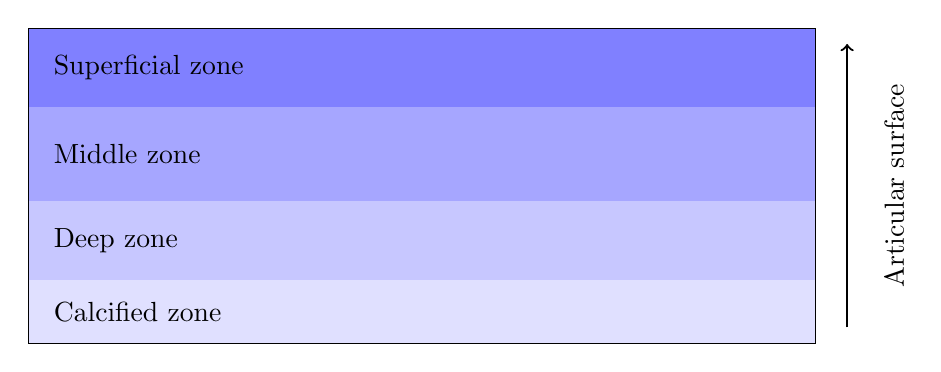
\begin{tikzpicture}[x=1cm,y=1cm]
    \fill[blue!12] (0,0) rectangle (10,0.8);
    \fill[blue!22] (0,0.8) rectangle (10,1.8);
    \fill[blue!35] (0,1.8) rectangle (10,3.0);
    \fill[blue!50] (0,3.0) rectangle (10,4.0);
    \draw (0,0) rectangle (10,4);
    \node[anchor=west] at (0.2,0.4) {Calcified zone};
    \node[anchor=west] at (0.2,1.3) {Deep zone};
    \node[anchor=west] at (0.2,2.4) {Middle zone};
    \node[anchor=west] at (0.2,3.5) {Superficial zone};
    \draw[->,thick] (10.4,0.2) -- (10.4,3.8);
    \node[rotate=90] at (11.0,2.0) {Articular surface};
  \end{tikzpicture}
  \caption{Schematic representation of the zones of articular cartilage}
  \label{fig:joint-model}
\end{figure}

\section{Research question}
State the primary research question and objectives. A simple mathematical
example is
\begin{equation}
  R = \alpha I + \beta M + \gamma S.
  \label{eq:risk}
\end{equation}

\begin{brightonquotation}
Indented quotations and footnotes may use single spacing under the Brighton
requirements.
\end{brightonquotation}

Equation~\ref{eq:risk} is numbered automatically and can be cited from any
chapter.

\subsection{Example objectives}
The description-list format is useful when each item needs a short label
followed by an explanation:

\begin{description}
  \item[Objective 1] Estimate the repeatability of the quantitative imaging
    measure under a prespecified acquisition protocol.
  \item[Objective 2] Test its association with change in symptoms and structure
    over 24 months.
  \item[Objective 3] Assess whether it adds useful predictive information to
    routinely available clinical variables.
\end{description}

\section{Chapter summary}
The chapter has demonstrated several paragraphs of ordinary prose, three levels
of numbered heading, ordered, unordered and description lists, two types of
figure, a quotation, a footnote, an equation and cross-references. The source
file remains independent from the other chapters while all numbering is
controlled by \texttt{main.tex}.

% !TeX root = ../main.tex
\chapter{Methods}

\section{Study design}
Describe the study population, sampling, imaging procedures, outcomes and
analysis plan. Table~\ref{tab:measures} demonstrates an ordinary floating table.
LaTeX supplies the chapter-based number and adds the caption to the list of
tables.

For illustration, assume a prospective cohort with baseline and 24-month
follow-up. Participants would undergo symptom assessment, clinical examination
and a standardised imaging protocol. An analysis plan written before outcome
assessment would identify the primary measure, expected confounders and approach
to missing observations.

\subsection{Eligibility}
An example set of inclusion criteria might require adults with knee symptoms
but no established radiographic disease. Exclusion criteria could include
contraindications to MRI, inflammatory arthritis, recent major trauma or
inability to complete follow-up.

\subsubsection{Recruitment pathway}
Potential participants could be identified through primary care, community
advertising or existing research cohorts. Screening should use the same written
criteria in every setting, and the number approached, assessed and enrolled
should be retained for the participant-flow diagram.

\subsubsection{Consent and withdrawal}
The information sheet should explain the imaging procedure, use of clinical
data, foreseeable burdens and the right to withdraw. The thesis should
distinguish withdrawal from further contact, withdrawal from future data
collection and any request concerning data already obtained.

\subsection{Imaging acquisition}
Scanner field strength, coils, positioning, sequences, voxel dimensions and
quality-control procedures should be reported sufficiently clearly for the
method to be reproduced.

\begin{table}[htbp]
  \caption{Example research measures}
  \label{tab:measures}
  \centering
  \begin{tabular}{lll}
    \toprule
    Domain & Measure & Purpose \\
    \midrule
    Imaging & Cartilage thickness & Structural change \\
    Clinical & Pain score & Patient experience \\
    Mechanical & Knee load & Physical exposure \\
    \bottomrule
  \end{tabular}
\end{table}

\section{Multi-page tables}
The \texttt{longtable} environment repeats its headings automatically when a
table crosses a page boundary. The short example below uses the same structure
and can be extended with additional rows.

\begin{longtable}{@{}p{0.22\textwidth}p{0.28\textwidth}p{0.38\textwidth}@{}}
\caption{Example data dictionary}
\label{tab:data-dictionary}\\
\toprule
Variable & Type & Description \\
\midrule
\endfirsthead

\multicolumn{3}{@{}l}{\tablename\ \thetable\ continued}\\
\toprule
Variable & Type & Description \\
\midrule
\endhead

\midrule
\multicolumn{3}{r@{}}{Continued on next page}\\
\endfoot

\bottomrule
\endlastfoot

Participant ID & Text & Pseudonymous study identifier. \\
Age & Number & Age at baseline assessment. \\
Pain score & Number & Patient-reported symptom measure. \\
Cartilage thickness & Number & Quantitative structural imaging measure. \\
T2 relaxation time & Number & Quantitative compositional imaging measure. \\
\end{longtable}

\section{Analysis}
Continuous variables could be summarised using means and standard deviations or
medians and interquartile ranges, depending on their distributions. Model
assumptions should be checked and uncertainty reported using confidence
intervals rather than relying only on thresholded significance tests.

\begin{equation}
  Y_{24} = \beta_0 + \beta_1 X_{\mathrm{MRI}}
           + \beta_2 Y_0 + \beta_3 A + \varepsilon,
  \label{eq:analysis-model}
\end{equation}

Equation~\ref{eq:analysis-model} illustrates a follow-up outcome adjusted for
baseline outcome \(Y_0\), age \(A\), and an MRI predictor.

\subsection{Sensitivity analyses}
Sensitivity analyses might repeat the primary model after alternative handling
of missing data, exclusion of scans that failed quality control and adjustment
for additional prespecified confounders. These analyses should test the
robustness of interpretation rather than act as a search for a preferred
result.

\subsection{Reporting}
Results should be presented with denominators, effect estimates and confidence
intervals. Tables should be understandable without repeatedly consulting the
main text, while the narrative should highlight the pattern of findings rather
than reproduce every number in the table.

\chapter{Results}

\section{Participant flow}
Figure~\ref{fig:flow} provides a second automatically numbered figure.

\begin{figure}[htbp]
  \centering
  \setlength{\unitlength}{1mm}
  \begin{picture}(90,55)
    \put(25,40){\framebox(40,10){120 assessed}}
    \put(45,40){\vector(0,-1){10}}
    \put(25,20){\framebox(40,10){100 recruited}}
    \put(45,20){\vector(0,-1){10}}
    \put(25,0){\framebox(40,10){92 analysed}}
  \end{picture}
  \caption{Illustrative participant flow through the study}
  \label{fig:flow}
\end{figure}

\section{Illustrative findings}
The hypothetical imaging measure changed between baseline and follow-up. Replace
this example with the actual analysis and its corresponding tables or figures.

\begin{table}[htbp]
  \caption{Illustrative baseline characteristics}
  \label{tab:baseline}
  \centering
  \begin{tabular}{lcc}
    \toprule
    Characteristic & Analysed sample & Missing \\
    \midrule
    Participants, \(n\) & 92 & -- \\
    Age, mean (SD), years & 57.4 (8.6) & 0 \\
    Female, \(n\) (\%) & 54 (58.7) & 0 \\
    Pain score, mean (SD) & 3.8 (1.9) & 2 \\
    Cartilage thickness, mean (SD), mm & 2.31 (0.28) & 4 \\
    \bottomrule
  \end{tabular}
\end{table}

Table~\ref{tab:baseline} shows the recommended practice of giving the table
number and title above the table. Units are included in the row labels, and
missingness is reported explicitly.

\section{Multi-panel figure}
Figure~\ref{fig:two-panel} demonstrates two panels within a single numbered
figure.

\begin{figure}[htbp]
  \centering
  \begin{subfigure}[t]{0.46\textwidth}
    \centering
    \begin{tikzpicture}[scale=0.85,transform shape]
      \draw[->] (0,0) -- (5.0,0) node[right] {Time};
      \draw[->] (0,0) -- (0,3.2) node[above] {Measure};
      \draw[blue,thick] plot[smooth] coordinates
        {(0.3,0.6) (1.2,0.9) (2.2,1.2) (3.2,1.8) (4.4,2.5)};
    \end{tikzpicture}
    \caption{Increasing trajectory}
  \end{subfigure}
  \hfill
  \begin{subfigure}[t]{0.46\textwidth}
    \centering
    \begin{tikzpicture}[scale=0.85,transform shape]
      \draw[->] (0,0) -- (5.0,0) node[right] {Time};
      \draw[->] (0,0) -- (0,3.2) node[above] {Measure};
      \draw[red!70!black,thick] plot[smooth] coordinates
        {(0.3,2.5) (1.2,2.1) (2.2,1.7) (3.2,1.1) (4.4,0.7)};
    \end{tikzpicture}
    \caption{Decreasing trajectory}
  \end{subfigure}
  \caption{Illustrative longitudinal trajectories shown as two panels}
  \label{fig:two-panel}
\end{figure}

\section{Result summary}
The example results chapter now contains a flow diagram, a conventional table
and a multi-panel vector figure. Actual analyses should report effect estimates,
uncertainty, denominators and missing data alongside clinically meaningful
interpretation.

\chapter{Discussion}

\section{Principal findings}
This example shows how the discussion can refer back to
Figure~\ref{fig:pathway}, Table~\ref{tab:measures} and
Equation~\ref{eq:risk} without manually entering their numbers.

\section{Strengths and limitations}
Interpret the findings, limitations and contribution to knowledge here.
Possible strengths include prospective data collection, prespecified outcomes,
standardised imaging and assessment of repeatability. Possible limitations
include selection bias, measurement error, loss to follow-up and limited
generalisability beyond the recruited population.

An endnote is useful for relevant background information that is not essential
to following the immediate argument.\endnote{This is an example endnote. Unlike
a footnote, it is collected in the dedicated Endnotes section near the end of
the thesis. Endnotes are numbered automatically in the order in which they are
called.}

\section{Implications}
The main implication of the hypothetical findings would depend on whether the
imaging measure improved prediction sufficiently to justify its cost and
complexity. Statistical association alone would not establish clinical utility.
Future studies might evaluate calibration, discrimination, decision consequences
and acceptability to patients.

\subsection{Implications for research}
Replication in an independent sample would test transportability. Longer
follow-up could establish whether an early imaging difference is transient or
marks a sustained disease trajectory. Studies should also compare the imaging
measure with simpler and less costly alternatives.

\subsection{Implications for practice}
Before clinical adoption, a biomarker requires a defined place in a care
pathway. Its benefit would depend on whether the result changes management and
whether that change improves an outcome that matters to patients without
creating disproportionate cost or burden.

\section{Chapter summary}
The discussion should return explicitly to the research questions, distinguish
findings from interpretation, acknowledge alternative explanations and identify
the precise contribution to knowledge.

\chapter{Conclusion}

The completed demonstration confirms that the modular files are combined into
one consecutively numbered thesis. Summarise the principal conclusions and
implications for research or practice here.

The template separates content from presentation: chapter files contain the
scholarly material, \texttt{main.tex} controls order and metadata, and
\texttt{brightonthesis.sty} contains the University formatting rules. This
separation allows future regulatory changes to be applied across the complete
thesis without editing hundreds of pages individually.

% !TeX root = ../main.tex
\chapter{Formatting Showcase}
\label{chap:formatting-showcase}

This chapter exists solely to make the template's features easy to inspect.
It can be deleted when beginning the real thesis. Every example is formatted
by \texttt{brightonthesis.sty}; the chapter file contains content and semantic
LaTeX commands, but no local margin, font or page-style settings.

The running header is visible above. It uses smaller type and shows the
candidate name, submission year and page number. It appears only in the
numbered main text. The formal page number is also retained at the bottom
centre. The option that enables the header is set near the top of
\texttt{main.tex}.

\section{Heading hierarchy}
\label{sec:showcase-headings}

Use headings to describe the structure of the argument. LaTeX calculates their
numbers, adds the required levels to the table of contents and updates
cross-references after compilation.

\subsection{A numbered subsection}
\label{sec:showcase-subsection}

This heading demonstrates the second level beneath a chapter. In a long thesis,
subsections help readers identify the distinct components of a method, result
or argument without making every short paragraph a separate section.

\subsubsection{A numbered subsubsection}
\label{sec:showcase-subsubsection}

This is the third displayed level beneath a chapter. The stylesheet gives it a
smaller, left-aligned heading while retaining automatic numbering. Use this
level sparingly so the hierarchy remains easy to follow.

\subsubsection{A second subsubsection}

The next heading number is generated automatically. If a section is moved to
another chapter, all its heading, figure, table and equation references update
after recompilation.

\subsection{Paragraphs and inline text}

Ordinary paragraphs are typed without formatting commands. A completely blank
line in the source begins a new paragraph. The stylesheet applies the approved
12-point font, one-and-a-half spacing, flush-left alignment and additional
space between paragraphs consistently across the thesis.

Use \emph{emphasis} for a term that needs modest emphasis and
\textbf{bold text} only where a strong visual distinction is genuinely useful.
File names and short pieces of code can be shown as
\texttt{chapters/06-formatting-showcase.tex}. A non-breaking space in a
reference, such as Figure~\ref{fig:showcase-pathway}, prevents the label and
number from being separated at a line ending.

\section{Lists}

Lists are useful when the items are genuinely parallel. They should not replace
connected explanatory prose simply to make the page look more varied.

\subsection{Bullet points}

The \texttt{itemize} environment creates bullet points:

\begin{itemize}
  \item define the population and sampling frame;
  \item describe acquisition and quality-control procedures;
  \item identify the primary and secondary outcomes;
  \item prespecify the statistical analysis; and
  \item report missing data and uncertainty.
\end{itemize}

Text following the list returns automatically to the ordinary paragraph style.
Punctuation is included here because the bullets form one continuing sentence.

\subsection{Numbered steps}

The \texttt{enumerate} environment is appropriate when order matters:

\begin{enumerate}
  \item Screen potential participants against the eligibility criteria.
  \item Obtain informed consent before research procedures begin.
  \item Acquire clinical and imaging measurements using the protocol.
  \item Perform quality control without reference to the later outcome.
  \item Conduct the prespecified analysis and report all relevant results.
\end{enumerate}

\subsection{Labelled descriptions}

A description list pairs a short label with explanatory text:

\begin{description}
  \item[Population] Adults with symptoms but without established radiographic
    osteoarthritis at baseline.
  \item[Exposure] A quantitative MRI measure obtained using a standardised
    acquisition and processing pipeline.
  \item[Outcome] Change in pain, function or structural status during follow-up.
\end{description}

\section{Figures and captions}

Figures are numbered by chapter, listed automatically in the list of figures
and referred to using labels. Captions appear below figures in accordance with
the Brighton guidance.

\subsection{Example figure one: process diagram}

Figure~\ref{fig:showcase-pathway} is a vector process diagram. Because it is
drawn in LaTeX, it remains sharp when enlarged in the PDF.

\begin{figure}[htbp]
  \centering
  \begin{tikzpicture}[
      node distance=1.1cm,
      every node/.style={font=\normalsize},
      box/.style={draw,rounded corners,minimum width=8.5cm,
        minimum height=1.05cm,align=center,fill=blue!8},
      arrow/.style={->,thick}
    ]
    \node[box] (question) {Research question and prespecified objectives};
    \node[box,below=of question] (measure) {Clinical and imaging measurements};
    \node[box,below=of measure] (analysis) {Quality control and statistical analysis};
    \node[box,below=of analysis] (interpret) {Interpretation and clinical relevance};
    \draw[arrow] (question) -- (measure);
    \draw[arrow] (measure) -- (analysis);
    \draw[arrow] (analysis) -- (interpret);
  \end{tikzpicture}
  \caption{Example pathway from research question to interpretation}
  \label{fig:showcase-pathway}
\end{figure}

\subsection{Example figure two: grouped observations}

Figure~\ref{fig:showcase-observations} demonstrates a second, visually distinct
figure and an automatically generated cross-reference.

\begin{figure}[htbp]
  \centering
  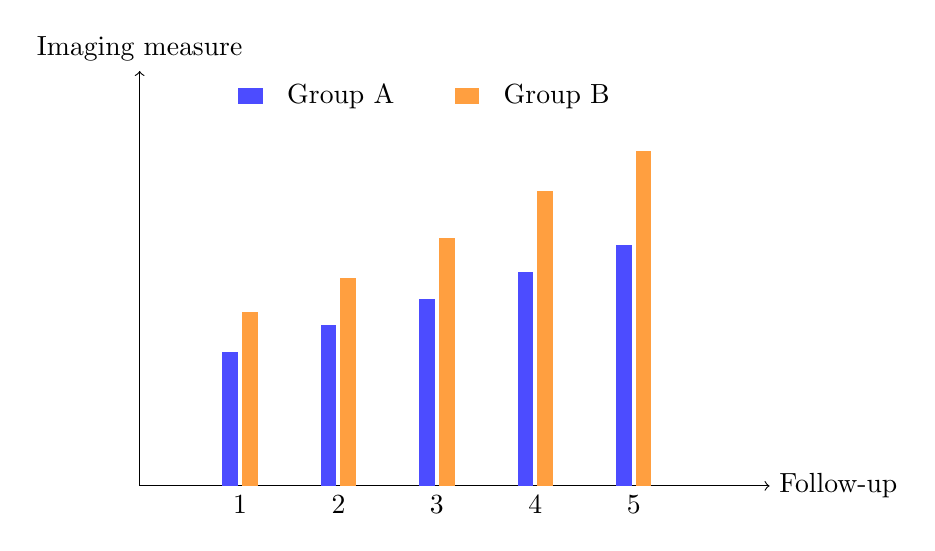
\begin{tikzpicture}[x=1.25cm,y=0.85cm]
    \draw[->] (0,0) -- (6.4,0) node[right] {Follow-up};
    \draw[->] (0,0) -- (0,6.2) node[above] {Imaging measure};
    \foreach \x/\a/\b in {1/2.0/2.6,2/2.4/3.1,3/2.8/3.7,4/3.2/4.4,5/3.6/5.0}
      {
        \fill[blue!70] (\x-0.16,0) rectangle (\x,{\a});
        \fill[orange!75] (\x+0.04,0) rectangle (\x+0.20,{\b});
      }
    \fill[blue!70] (1.0,5.7) rectangle (1.25,5.95);
    \node[anchor=west] at (1.4,5.82) {Group A};
    \fill[orange!75] (3.2,5.7) rectangle (3.45,5.95);
    \node[anchor=west] at (3.6,5.82) {Group B};
    \foreach \x in {1,...,5} \node[below] at (\x+0.02,0) {\x};
  \end{tikzpicture}
  \caption{Illustrative grouped measurements over five follow-up occasions}
  \label{fig:showcase-observations}
\end{figure}

When using an external image instead, place the image in a
\texttt{figures/} folder and replace the drawing code with
\verb|\includegraphics|, as shown in the README.

\section{Table, equation and quotation}

\subsection{Example table}

Table~\ref{tab:showcase-measures} has its number and title above the table.
The row and column headings include enough information for the example to be
understood independently of the surrounding paragraph.

\begin{table}[htbp]
  \caption{Illustrative measurements and reporting formats}
  \label{tab:showcase-measures}
  \centering
  \begin{tabular}{lll}
    \toprule
    Domain & Example measure & Reporting format \\
    \midrule
    Symptoms & Pain score & Mean (SD) \\
    Structure & Cartilage thickness & Millimetres \\
    Composition & T2 relaxation time & Milliseconds \\
    Function & Walking speed & Metres per second \\
    \bottomrule
  \end{tabular}
\end{table}

\subsection{Example equation}

Numbered equations can be referenced in the same way as figures and tables:
\begin{equation}
  \Delta Y = Y_{\mathrm{follow\text{-}up}} - Y_{\mathrm{baseline}}.
  \label{eq:showcase-change}
\end{equation}
Equation~\ref{eq:showcase-change} defines a simple change score. Short
mathematical expressions such as \(n=120\) can also appear within a sentence.

\subsection{Example quotation}

\begin{brightonquotation}
This indented passage demonstrates the single-spaced quotation environment.
Replace it with the quoted material, include a page number where appropriate
and provide the corresponding citation.
\end{brightonquotation}

\section{Footnote and endnote examples}

A footnote marker appears here.\footnote{This is a visible example footnote.
It is numbered automatically and printed at the bottom of the same page in
smaller, single-spaced text.} Footnotes should contain information needed to
understand the nearby text without interrupting the main sentence.

An endnote marker appears here.\endnote{This second example endnote was called
from the formatting-showcase chapter. It is collected with the earlier
endnote in the dedicated Endnotes section near the end of the thesis.}
The superscript marker beside the preceding sentence points to the numbered
entry printed in the separate \emph{Endnotes} section. It is not printed at
the bottom of this page. Endnotes are useful for additional material that can
be read separately from the immediate argument.

\section{Cross-references and chapter summary}

This chapter referred to Section~\ref{sec:showcase-headings},
Figure~\ref{fig:showcase-pathway}, Figure~\ref{fig:showcase-observations},
Table~\ref{tab:showcase-measures} and Equation~\ref{eq:showcase-change} without
typing their final numbers. The labels remain stable even if the content moves.

The source demonstrates running headings, multiple heading levels, ordinary
paragraphs, inline formatting, bullet points, numbered steps, description
lists, two figures, a table, an equation, a quotation, a footnote, an endnote
and cross-references. Delete the line
\verb|% !TeX root = ../main.tex
\chapter{Formatting Showcase}
\label{chap:formatting-showcase}

This chapter exists solely to make the template's features easy to inspect.
It can be deleted when beginning the real thesis. Every example is formatted
by \texttt{brightonthesis.sty}; the chapter file contains content and semantic
LaTeX commands, but no local margin, font or page-style settings.

The running header is visible above. It uses smaller type and shows the
candidate name, submission year and page number. It appears only in the
numbered main text. The formal page number is also retained at the bottom
centre. The option that enables the header is set near the top of
\texttt{main.tex}.

\section{Heading hierarchy}
\label{sec:showcase-headings}

Use headings to describe the structure of the argument. LaTeX calculates their
numbers, adds the required levels to the table of contents and updates
cross-references after compilation.

\subsection{A numbered subsection}
\label{sec:showcase-subsection}

This heading demonstrates the second level beneath a chapter. In a long thesis,
subsections help readers identify the distinct components of a method, result
or argument without making every short paragraph a separate section.

\subsubsection{A numbered subsubsection}
\label{sec:showcase-subsubsection}

This is the third displayed level beneath a chapter. The stylesheet gives it a
smaller, left-aligned heading while retaining automatic numbering. Use this
level sparingly so the hierarchy remains easy to follow.

\subsubsection{A second subsubsection}

The next heading number is generated automatically. If a section is moved to
another chapter, all its heading, figure, table and equation references update
after recompilation.

\subsection{Paragraphs and inline text}

Ordinary paragraphs are typed without formatting commands. A completely blank
line in the source begins a new paragraph. The stylesheet applies the approved
12-point font, one-and-a-half spacing, flush-left alignment and additional
space between paragraphs consistently across the thesis.

Use \emph{emphasis} for a term that needs modest emphasis and
\textbf{bold text} only where a strong visual distinction is genuinely useful.
File names and short pieces of code can be shown as
\texttt{chapters/06-formatting-showcase.tex}. A non-breaking space in a
reference, such as Figure~\ref{fig:showcase-pathway}, prevents the label and
number from being separated at a line ending.

\section{Lists}

Lists are useful when the items are genuinely parallel. They should not replace
connected explanatory prose simply to make the page look more varied.

\subsection{Bullet points}

The \texttt{itemize} environment creates bullet points:

\begin{itemize}
  \item define the population and sampling frame;
  \item describe acquisition and quality-control procedures;
  \item identify the primary and secondary outcomes;
  \item prespecify the statistical analysis; and
  \item report missing data and uncertainty.
\end{itemize}

Text following the list returns automatically to the ordinary paragraph style.
Punctuation is included here because the bullets form one continuing sentence.

\subsection{Numbered steps}

The \texttt{enumerate} environment is appropriate when order matters:

\begin{enumerate}
  \item Screen potential participants against the eligibility criteria.
  \item Obtain informed consent before research procedures begin.
  \item Acquire clinical and imaging measurements using the protocol.
  \item Perform quality control without reference to the later outcome.
  \item Conduct the prespecified analysis and report all relevant results.
\end{enumerate}

\subsection{Labelled descriptions}

A description list pairs a short label with explanatory text:

\begin{description}
  \item[Population] Adults with symptoms but without established radiographic
    osteoarthritis at baseline.
  \item[Exposure] A quantitative MRI measure obtained using a standardised
    acquisition and processing pipeline.
  \item[Outcome] Change in pain, function or structural status during follow-up.
\end{description}

\section{Figures and captions}

Figures are numbered by chapter, listed automatically in the list of figures
and referred to using labels. Captions appear below figures in accordance with
the Brighton guidance.

\subsection{Example figure one: process diagram}

Figure~\ref{fig:showcase-pathway} is a vector process diagram. Because it is
drawn in LaTeX, it remains sharp when enlarged in the PDF.

\begin{figure}[htbp]
  \centering
  \begin{tikzpicture}[
      node distance=1.1cm,
      every node/.style={font=\normalsize},
      box/.style={draw,rounded corners,minimum width=8.5cm,
        minimum height=1.05cm,align=center,fill=blue!8},
      arrow/.style={->,thick}
    ]
    \node[box] (question) {Research question and prespecified objectives};
    \node[box,below=of question] (measure) {Clinical and imaging measurements};
    \node[box,below=of measure] (analysis) {Quality control and statistical analysis};
    \node[box,below=of analysis] (interpret) {Interpretation and clinical relevance};
    \draw[arrow] (question) -- (measure);
    \draw[arrow] (measure) -- (analysis);
    \draw[arrow] (analysis) -- (interpret);
  \end{tikzpicture}
  \caption{Example pathway from research question to interpretation}
  \label{fig:showcase-pathway}
\end{figure}

\subsection{Example figure two: grouped observations}

Figure~\ref{fig:showcase-observations} demonstrates a second, visually distinct
figure and an automatically generated cross-reference.

\begin{figure}[htbp]
  \centering
  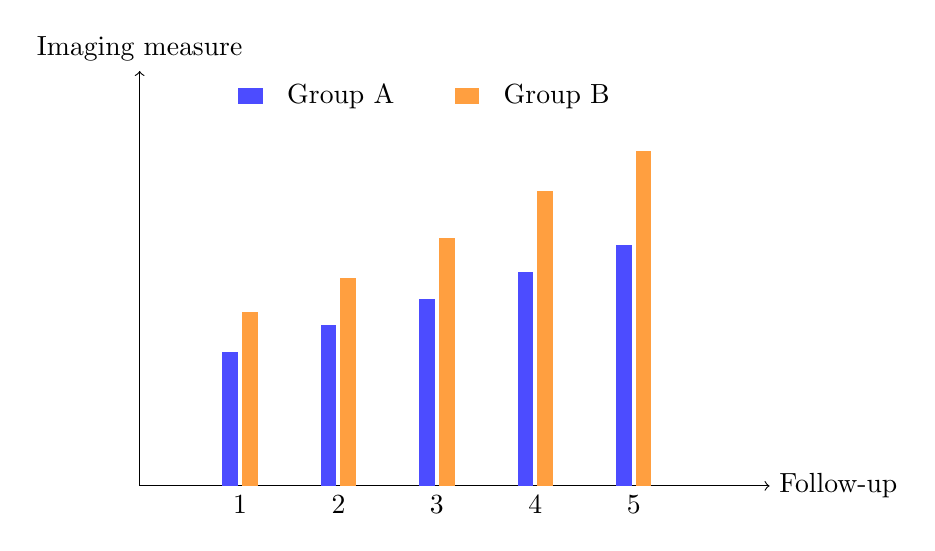
\begin{tikzpicture}[x=1.25cm,y=0.85cm]
    \draw[->] (0,0) -- (6.4,0) node[right] {Follow-up};
    \draw[->] (0,0) -- (0,6.2) node[above] {Imaging measure};
    \foreach \x/\a/\b in {1/2.0/2.6,2/2.4/3.1,3/2.8/3.7,4/3.2/4.4,5/3.6/5.0}
      {
        \fill[blue!70] (\x-0.16,0) rectangle (\x,{\a});
        \fill[orange!75] (\x+0.04,0) rectangle (\x+0.20,{\b});
      }
    \fill[blue!70] (1.0,5.7) rectangle (1.25,5.95);
    \node[anchor=west] at (1.4,5.82) {Group A};
    \fill[orange!75] (3.2,5.7) rectangle (3.45,5.95);
    \node[anchor=west] at (3.6,5.82) {Group B};
    \foreach \x in {1,...,5} \node[below] at (\x+0.02,0) {\x};
  \end{tikzpicture}
  \caption{Illustrative grouped measurements over five follow-up occasions}
  \label{fig:showcase-observations}
\end{figure}

When using an external image instead, place the image in a
\texttt{figures/} folder and replace the drawing code with
\verb|\includegraphics|, as shown in the README.

\section{Table, equation and quotation}

\subsection{Example table}

Table~\ref{tab:showcase-measures} has its number and title above the table.
The row and column headings include enough information for the example to be
understood independently of the surrounding paragraph.

\begin{table}[htbp]
  \caption{Illustrative measurements and reporting formats}
  \label{tab:showcase-measures}
  \centering
  \begin{tabular}{lll}
    \toprule
    Domain & Example measure & Reporting format \\
    \midrule
    Symptoms & Pain score & Mean (SD) \\
    Structure & Cartilage thickness & Millimetres \\
    Composition & T2 relaxation time & Milliseconds \\
    Function & Walking speed & Metres per second \\
    \bottomrule
  \end{tabular}
\end{table}

\subsection{Example equation}

Numbered equations can be referenced in the same way as figures and tables:
\begin{equation}
  \Delta Y = Y_{\mathrm{follow\text{-}up}} - Y_{\mathrm{baseline}}.
  \label{eq:showcase-change}
\end{equation}
Equation~\ref{eq:showcase-change} defines a simple change score. Short
mathematical expressions such as \(n=120\) can also appear within a sentence.

\subsection{Example quotation}

\begin{brightonquotation}
This indented passage demonstrates the single-spaced quotation environment.
Replace it with the quoted material, include a page number where appropriate
and provide the corresponding citation.
\end{brightonquotation}

\section{Footnote and endnote examples}

A footnote marker appears here.\footnote{This is a visible example footnote.
It is numbered automatically and printed at the bottom of the same page in
smaller, single-spaced text.} Footnotes should contain information needed to
understand the nearby text without interrupting the main sentence.

An endnote marker appears here.\endnote{This second example endnote was called
from the formatting-showcase chapter. It is collected with the earlier
endnote in the dedicated Endnotes section near the end of the thesis.}
The superscript marker beside the preceding sentence points to the numbered
entry printed in the separate \emph{Endnotes} section. It is not printed at
the bottom of this page. Endnotes are useful for additional material that can
be read separately from the immediate argument.

\section{Cross-references and chapter summary}

This chapter referred to Section~\ref{sec:showcase-headings},
Figure~\ref{fig:showcase-pathway}, Figure~\ref{fig:showcase-observations},
Table~\ref{tab:showcase-measures} and Equation~\ref{eq:showcase-change} without
typing their final numbers. The labels remain stable even if the content moves.

The source demonstrates running headings, multiple heading levels, ordinary
paragraphs, inline formatting, bullet points, numbered steps, description
lists, two figures, a table, an equation, a quotation, a footnote, an endnote
and cross-references. Delete the line
\verb|% !TeX root = ../main.tex
\chapter{Formatting Showcase}
\label{chap:formatting-showcase}

This chapter exists solely to make the template's features easy to inspect.
It can be deleted when beginning the real thesis. Every example is formatted
by \texttt{brightonthesis.sty}; the chapter file contains content and semantic
LaTeX commands, but no local margin, font or page-style settings.

The running header is visible above. It uses smaller type and shows the
candidate name, submission year and page number. It appears only in the
numbered main text. The formal page number is also retained at the bottom
centre. The option that enables the header is set near the top of
\texttt{main.tex}.

\section{Heading hierarchy}
\label{sec:showcase-headings}

Use headings to describe the structure of the argument. LaTeX calculates their
numbers, adds the required levels to the table of contents and updates
cross-references after compilation.

\subsection{A numbered subsection}
\label{sec:showcase-subsection}

This heading demonstrates the second level beneath a chapter. In a long thesis,
subsections help readers identify the distinct components of a method, result
or argument without making every short paragraph a separate section.

\subsubsection{A numbered subsubsection}
\label{sec:showcase-subsubsection}

This is the third displayed level beneath a chapter. The stylesheet gives it a
smaller, left-aligned heading while retaining automatic numbering. Use this
level sparingly so the hierarchy remains easy to follow.

\subsubsection{A second subsubsection}

The next heading number is generated automatically. If a section is moved to
another chapter, all its heading, figure, table and equation references update
after recompilation.

\subsection{Paragraphs and inline text}

Ordinary paragraphs are typed without formatting commands. A completely blank
line in the source begins a new paragraph. The stylesheet applies the approved
12-point font, one-and-a-half spacing, flush-left alignment and additional
space between paragraphs consistently across the thesis.

Use \emph{emphasis} for a term that needs modest emphasis and
\textbf{bold text} only where a strong visual distinction is genuinely useful.
File names and short pieces of code can be shown as
\texttt{chapters/06-formatting-showcase.tex}. A non-breaking space in a
reference, such as Figure~\ref{fig:showcase-pathway}, prevents the label and
number from being separated at a line ending.

\section{Lists}

Lists are useful when the items are genuinely parallel. They should not replace
connected explanatory prose simply to make the page look more varied.

\subsection{Bullet points}

The \texttt{itemize} environment creates bullet points:

\begin{itemize}
  \item define the population and sampling frame;
  \item describe acquisition and quality-control procedures;
  \item identify the primary and secondary outcomes;
  \item prespecify the statistical analysis; and
  \item report missing data and uncertainty.
\end{itemize}

Text following the list returns automatically to the ordinary paragraph style.
Punctuation is included here because the bullets form one continuing sentence.

\subsection{Numbered steps}

The \texttt{enumerate} environment is appropriate when order matters:

\begin{enumerate}
  \item Screen potential participants against the eligibility criteria.
  \item Obtain informed consent before research procedures begin.
  \item Acquire clinical and imaging measurements using the protocol.
  \item Perform quality control without reference to the later outcome.
  \item Conduct the prespecified analysis and report all relevant results.
\end{enumerate}

\subsection{Labelled descriptions}

A description list pairs a short label with explanatory text:

\begin{description}
  \item[Population] Adults with symptoms but without established radiographic
    osteoarthritis at baseline.
  \item[Exposure] A quantitative MRI measure obtained using a standardised
    acquisition and processing pipeline.
  \item[Outcome] Change in pain, function or structural status during follow-up.
\end{description}

\section{Figures and captions}

Figures are numbered by chapter, listed automatically in the list of figures
and referred to using labels. Captions appear below figures in accordance with
the Brighton guidance.

\subsection{Example figure one: process diagram}

Figure~\ref{fig:showcase-pathway} is a vector process diagram. Because it is
drawn in LaTeX, it remains sharp when enlarged in the PDF.

\begin{figure}[htbp]
  \centering
  \begin{tikzpicture}[
      node distance=1.1cm,
      every node/.style={font=\normalsize},
      box/.style={draw,rounded corners,minimum width=8.5cm,
        minimum height=1.05cm,align=center,fill=blue!8},
      arrow/.style={->,thick}
    ]
    \node[box] (question) {Research question and prespecified objectives};
    \node[box,below=of question] (measure) {Clinical and imaging measurements};
    \node[box,below=of measure] (analysis) {Quality control and statistical analysis};
    \node[box,below=of analysis] (interpret) {Interpretation and clinical relevance};
    \draw[arrow] (question) -- (measure);
    \draw[arrow] (measure) -- (analysis);
    \draw[arrow] (analysis) -- (interpret);
  \end{tikzpicture}
  \caption{Example pathway from research question to interpretation}
  \label{fig:showcase-pathway}
\end{figure}

\subsection{Example figure two: grouped observations}

Figure~\ref{fig:showcase-observations} demonstrates a second, visually distinct
figure and an automatically generated cross-reference.

\begin{figure}[htbp]
  \centering
  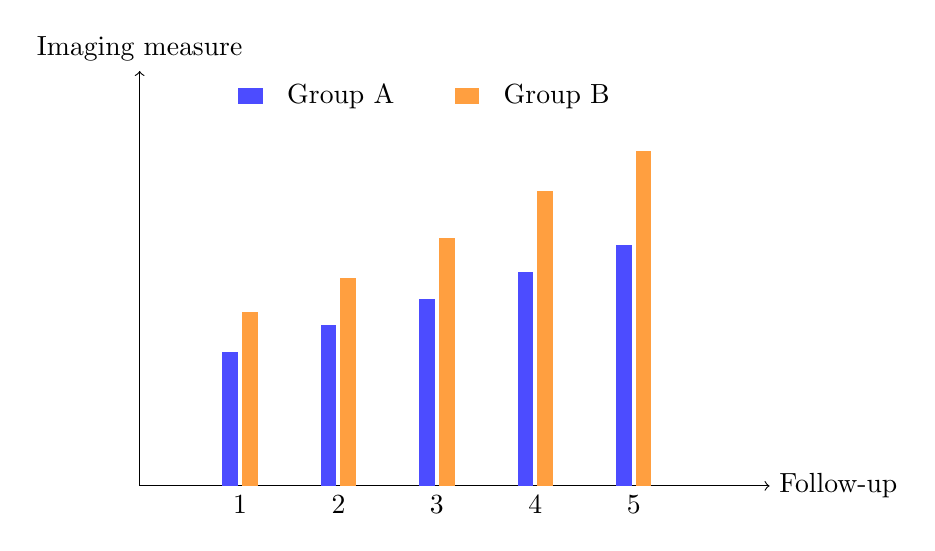
\begin{tikzpicture}[x=1.25cm,y=0.85cm]
    \draw[->] (0,0) -- (6.4,0) node[right] {Follow-up};
    \draw[->] (0,0) -- (0,6.2) node[above] {Imaging measure};
    \foreach \x/\a/\b in {1/2.0/2.6,2/2.4/3.1,3/2.8/3.7,4/3.2/4.4,5/3.6/5.0}
      {
        \fill[blue!70] (\x-0.16,0) rectangle (\x,{\a});
        \fill[orange!75] (\x+0.04,0) rectangle (\x+0.20,{\b});
      }
    \fill[blue!70] (1.0,5.7) rectangle (1.25,5.95);
    \node[anchor=west] at (1.4,5.82) {Group A};
    \fill[orange!75] (3.2,5.7) rectangle (3.45,5.95);
    \node[anchor=west] at (3.6,5.82) {Group B};
    \foreach \x in {1,...,5} \node[below] at (\x+0.02,0) {\x};
  \end{tikzpicture}
  \caption{Illustrative grouped measurements over five follow-up occasions}
  \label{fig:showcase-observations}
\end{figure}

When using an external image instead, place the image in a
\texttt{figures/} folder and replace the drawing code with
\verb|\includegraphics|, as shown in the README.

\section{Table, equation and quotation}

\subsection{Example table}

Table~\ref{tab:showcase-measures} has its number and title above the table.
The row and column headings include enough information for the example to be
understood independently of the surrounding paragraph.

\begin{table}[htbp]
  \caption{Illustrative measurements and reporting formats}
  \label{tab:showcase-measures}
  \centering
  \begin{tabular}{lll}
    \toprule
    Domain & Example measure & Reporting format \\
    \midrule
    Symptoms & Pain score & Mean (SD) \\
    Structure & Cartilage thickness & Millimetres \\
    Composition & T2 relaxation time & Milliseconds \\
    Function & Walking speed & Metres per second \\
    \bottomrule
  \end{tabular}
\end{table}

\subsection{Example equation}

Numbered equations can be referenced in the same way as figures and tables:
\begin{equation}
  \Delta Y = Y_{\mathrm{follow\text{-}up}} - Y_{\mathrm{baseline}}.
  \label{eq:showcase-change}
\end{equation}
Equation~\ref{eq:showcase-change} defines a simple change score. Short
mathematical expressions such as \(n=120\) can also appear within a sentence.

\subsection{Example quotation}

\begin{brightonquotation}
This indented passage demonstrates the single-spaced quotation environment.
Replace it with the quoted material, include a page number where appropriate
and provide the corresponding citation.
\end{brightonquotation}

\section{Footnote and endnote examples}

A footnote marker appears here.\footnote{This is a visible example footnote.
It is numbered automatically and printed at the bottom of the same page in
smaller, single-spaced text.} Footnotes should contain information needed to
understand the nearby text without interrupting the main sentence.

An endnote marker appears here.\endnote{This second example endnote was called
from the formatting-showcase chapter. It is collected with the earlier
endnote in the dedicated Endnotes section near the end of the thesis.}
The superscript marker beside the preceding sentence points to the numbered
entry printed in the separate \emph{Endnotes} section. It is not printed at
the bottom of this page. Endnotes are useful for additional material that can
be read separately from the immediate argument.

\section{Cross-references and chapter summary}

This chapter referred to Section~\ref{sec:showcase-headings},
Figure~\ref{fig:showcase-pathway}, Figure~\ref{fig:showcase-observations},
Table~\ref{tab:showcase-measures} and Equation~\ref{eq:showcase-change} without
typing their final numbers. The labels remain stable even if the content moves.

The source demonstrates running headings, multiple heading levels, ordinary
paragraphs, inline formatting, bullet points, numbered steps, description
lists, two figures, a table, an equation, a quotation, a footnote, an endnote
and cross-references. Delete the line
\verb|\include{chapters/06-formatting-showcase}| from \texttt{main.tex} when
this demonstration is no longer required.
| from \texttt{main.tex} when
this demonstration is no longer required.
| from \texttt{main.tex} when
this demonstration is no longer required.


% ---------- END PAGES ----------
\brightonfrontmatterstyle
\brightonfrontchapter{Endnotes}

% The endnotes package normally creates its own heading. The template already
% created the correctly formatted chapter heading above.
\renewcommand{\enoteheading}{}
\theendnotes

\brightonfrontchapter{Glossary}

\begin{description}
  \item[Articular cartilage] The specialised connective tissue covering the
  ends of bones in synovial joints.
  \item[Quantitative imaging] Imaging methods that produce numerical measures
  of tissue structure or composition.
\end{description}


\ifbrightonbiblatex
  \printbibliography[heading=bibintoc,title={List of references}]
\else
  \brightonfrontchapter{List of references}
  \begin{thebibliography}{9}
    \bibitem{example2026}
    Example Author (2026).
    \newblock Early imaging and joint health.
    \newblock \emph{Journal of Demonstration Studies}, 1(1), 1--10.
  \end{thebibliography}
\fi


\brightonfrontchapter{Bibliography}

Include works consulted but not cited if your discipline requires a separate
bibliography. Otherwise delete this file and its corresponding
\texttt{\string\include} line in \texttt{main.tex}.



\appendix
\chapter{Supplementary material}

\section{Example appendix section}
Appendix chapters are lettered automatically. Add supplementary methods, tables,
questionnaires or other material here.


\end{document}
